\documentclass[conference]{IEEEtran}
\IEEEoverridecommandlockouts
\usepackage{cite}
\usepackage{amsmath,amssymb,amsfonts}
\usepackage{algorithmic}
\usepackage{mathpazo}
\usepackage[spanish]{babel}
\usepackage[utf8]{inputenc}
\usepackage[T1]{fontenc}
\usepackage{graphicx}
\usepackage{textcomp}
\usepackage{xcolor}
%\usepackage{minted}
%\usemintedstyle{emacs}
\usepackage{url}
\usepackage{ctable}
\usepackage{float}
\usepackage{amsmath,amssymb,amsfonts}
\usepackage{makecell}
\usepackage{hyperref}
\usepackage{comment}
\hypersetup{
	colorlinks=true,
	linkcolor=blue,
	filecolor=magenta,      
	urlcolor=cyan,
}
\newcommand{\DNoise}{n_d}

\newcommand{\Est}[1]{\hat{#1}}
\newcommand{\Test}[1]{\expandafter\hat#1}

\def\BibTeX{{\rm B\kern-.05em{\sc i\kern-.025em b}\kern-.08em
    T\kern-.1667em\lower.7ex\hbox{E}\kern-.125emX}}
    
\begin{document}
\title{\bf{Consultas SparQl a Estructuras RDF}}

\begin{comment}
\author{\IEEEauthorblockN{Asmat Franco, Bryan}
\IEEEauthorblockA{\textit{Universidad Nacional de Ingeniería} \\
Lima, Perú \\
\texttt{basmatf@uni.pe}}
\and
\IEEEauthorblockN{Blas Salas, Israel}
\IEEEauthorblockA{\textit{Universidad Nacional de Ingeniería} \\
Lima, Perú \\
\texttt{iblass@uni.pe}}
\and
\IEEEauthorblockN{Chavez Bruno, Victor}
\IEEEauthorblockA{\textit{Universidad Nacional de Ingeniería} \\
Lima, Perú \\
\texttt{vchavezb@uni.pe}}
\and
\IEEEauthorblockN{Guadalupe Quispe, William}
\IEEEauthorblockA{\textit{Universidad Nacional de Ingenieri\'a} \\
Lima, Perú \\
\texttt{wguadalupeq@uni.pe}}
}
\end{comment}
\author{%x  x
\textsc{Bryan Asmat}\textsc{, Danilo Blas}\textsc{, Victor Chavez}\textsc{, William Guadalupe}\\
%\thanks{A thank you or further information} \\[1ex] % Your name
\normalsize Universidad Nacional de Ingeniería \\ % Your institution
\normalsize Lima,Perú \\ % Your institution
\normalsize \href{mailto:basmatf@uni.pe}{basmatf@uni.pe},  \href{mailto:iblass@uni.pe}{iblass@uni.pe} \href{mailto:vchavezb@uni.pe}{,  vchavezb@uni.pe} \href{mailto:wguadalupeq@uni.pe}{,  wguadalupeq@uni.pe} % Your email address
%\and % Uncomment if 2 authors are required, duplicate these 4 lines if more
%\textsc{Jane Smith}\thanks{Corresponding author} \\[1ex] % Second author's name
%\normalsize University of Utah \\ % Second author's institution
%\normalsize \href{mailto:jane@smith.com}{jane@smith.com} % Second author's email address
}





\maketitle

\begin{abstract}
En el presente trabajo se implementaron consultas de tipos SparQL que permiten hacer la búsqueda en distintas fuentes de datos como estructuras RDF,la creación de esta estructura, asi como un resumen de los pasos que realizamos para la ejecución del proyecto.

Para iniciar el proyecto se usó la base de conocimiento de la Wikidata realizando consultas online \textbf{https://query.wikidata.org/} con lo cual seguiremos los siguientes pasos para que se entienda como se ha creado la estructura RDF.
\vspace{0.2cm}
Accedemos al enlace mencionado anteriormente.Podemos usar las consultas con extensión .rq que estan almacenadas en el repositorio de este proyecto:
\vspace{0.2cm}
Si usamos el contenido del archivo onlineQuerySELECT.rq copiaremos la información y la usaremos en el servicio de consultas de la Wikidata nos devuelve la tabla que hemos construido mediante las consultas que hemos hecho.
Si usamos el contenido del archivo onlineQueryCONSTRUCT.rq copiaremos la información y la usaremos en el servicio de consultas de la Wikidata nos devuelve como serían las tripletas en una nueva estructura RDF que vamos a manejar.
\vspace{0.2cm}
Descargamos el archivo TSV detallado que se genera al usar el archivo onlineQueryCONSTRUCT.rq y lo modificamos para que tenga el formato Turtle a usar en el presente proyecto.
El archivo RDF en formato turtle una vez generado y se encuentra en el siguiente en el directorio RDF con el siguiente nombre RDF.ttl.
\vspace{0.2cm}
Hasta ahora los pasos que hemos hecho es para extraer una estructura RDF nueva de Wikidata realizado consultas SparQL para obtener datos de investigaciones y trabajos científicos, digamos obras, que se basen sobre el tema de Ciencias de la Computación. De estos datos hemos extraído las siguiente características:

Titulo,Autor,Tema, Idioma, Revista,  Fecha de Publicación, URL.

\vspace{0.2cm}


\end{abstract}

\section{Introducci\'on}
\vspace{0.2cm}
La información en la web se puede representar bajo un formato de datos llamado RDF.
El consorcio World Wide Web (W3C) propuso una especificación llamada SparQL(lenguaje de consultas) para manipular grafos compuesstos por tripletas RDF en la web y en repositorios de datos, asi como extraer datos mediante consultas a relaciones desconocidas  y relaizar búsquedas con combinaciones complejas de base de datos.

\vspace{0.5cm}
La estructura de los resultados de una consulta SPARQL es una tabla donde cada fila es un resultado y cada columna se corresponde con una de las variables de la consulta.

Una consulta SparQL consta de tres partes:
\begin{itemize}
    \item  Coincidencia de patrones: optional, union, nesting,filtering.
    \item  Modificadores de solución: projection, distinct, order, límit, offset.
    \item  Parte de salida: construcción de nuevas tripletas.
\end{itemize}

\vspace{0.5cm}
Las búsquedas se realizan a través de un SparQL Endpoint, que es la interfaz de entrada y salida de estas bases de datos y que permitirá nuestras consultas. Dicho de otra forma, los Endpoints de SparQL no son más que una dirección web (URL) que acepta peticiones de búsqueda SparQL y devuelve resultados, las formas de consulta SparQL son select, construct, ask y describe.

\vspace{0.5cm}
\textbf{¿Cuáles son los desafíos de diseño en SparQL?}
\vspace{0.5cm}

SparQL debe tener en cuenta las características distintivas de RDF:
\begin{itemize}
    \item Debería poder extraer información de grafos RDF interconectados.
    \item Debe ser coherente con la semántica de mundo abierto de RDF.
    \item Debe ofrecer la posibilidad de agregar información opcional si está presente. 
    \item Debería ser capaz de interpretar correctamente grafos RDF con un vocabulario con semántica predefinida.
    \item Debería ofrecer algunas funcionalidades para navegar en un grafo RDF.
\end{itemize}

\vspace{0.2cm}

\section{¿Que es la web Semántica?}

La Web Semántica vendría a ser una extensión de la Web actual dotada de significado, esto es, un espacio donde la información tendría un significado bien definido, de manera que pudiera ser interpretada tanto por agentes humanos como por agentes computarizados.

\vspace{0.2cm}

La web Semántica ha sido impulsada, entre otros, por el creador de la web, Tim Berners Lee en el 2000 para que la información sea reunida de forma que los buscadores puedan ''comprender'', más allá de limitarse a colocar los documentos en una lista

\begin{figure}[h]
%	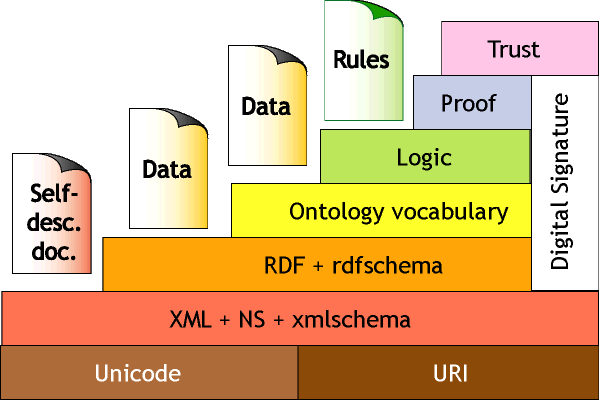
\includegraphics[scale=0.25]{imagenes/imagen1.jpg} 
	\caption{Transformer XL: Entrenamiento y Evaluación. Fuente: Transformer XL \cite{b7}}
\end{figure}

\section{URLs, URIs, IRIs}
\subsection{URLs}
El LRU es una cadena de caracteres con la que se asigna una dirección única a cada uno de los recursos de información disponibles en Internet. Existe un URL único para cada página de cada uno de los documentos de la WWW

\subsection{URIs}
Un identificador de recursos uniforme es una cadena de caracteres que identifica los recursos de una red de forma unívoca. La diferencia respecto a un localizador de recursos uniforme (URL) es que estos últimos hacen referencia a recursos que, de forma general, pueden variar en el tiempo. 

Normalmente estos recursos son accesibles en una red o sistema. Los URI pueden ser localizador de recursos uniforme (URL),(URN)
\subsection{IRIs}
Es un estándar de protocolo de Internet que se basa en el protocolo Identificador uniforme de recursos (URI) al expandir en gran medida el conjunto de caracteres permitidos.

\section{Estructura RDF}
RDF es un método general para descomponer cualquier tipo de conocimiento en trozos pequeños, con algunas reglas acerca de la semántica o significado, de esas piezas.

El punto es tener un método tan simple que puede expresar cualquier hecho, y a la vez tan estructurada que las aplicaciones informáticas pueden hacer cosas útiles con él. \textcolor{orange}{Attention Is All You Need} \cite{b1}

RDF representa la información en una declaración triple -también llamada tripleta- que sigue la estructura sujeto-predicado-objeto \textcolor{orange}{Aqui citaremos las paginas} \cite{b1}

\vspace{0.2cm}
\textbf{Ejemplo}

<La ronda de noche> <fue creada por> <Rembrandt>
\vspace{0.2cm}
En este ejemplo\textbf{<La ronda de noche>} y el objeto \textbf{<Rembrandt>} se pueden considerar como dos nodos en un grafo donde el predicado \textbf{<fue creada por>} define una arista o la relación entre estos .

\vspace{0.2cm}

\begin{figure}[h]
    \centering
	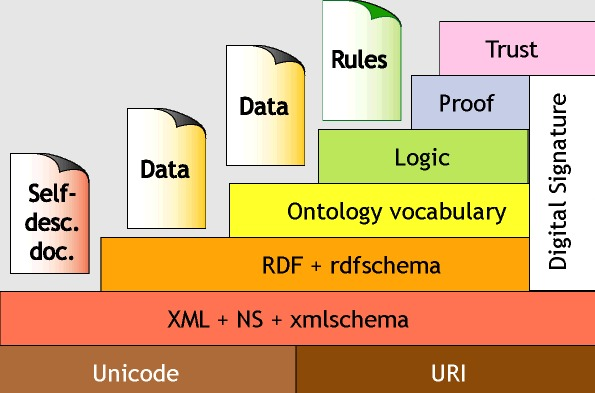
\includegraphics[scale=0.40]{imagenes/imagen1.jpeg} 
	\caption{Web semántica \cite{b7}}
\end{figure}

\vspace{0.2cm}




\vspace{0.2cm}

\section{Buscando RDF con SPARQL}
SPARQL nos permite traducir datos en grafo, intensamente enlazados, en datos normalizados en formato tabular, esto es, distribuidos en filas y columnas, que se pueden abrir  en formato como .csv .json .ttl ,etc o también se pueden ver en programas de visualización


Resulta útil pensar las consultas SPARQL como un conjunto de oraciones con espacios en blanco. La base de datos tomará esta consulta y encontrará cada conjunto de oraciones que encaje correctamente en estos espacios en blanco, devolviéndonos los valores coincidentes como una tabla.
\vspace{0.2cm}




\section{Consultas SPARQL}


SPARQL, acrónimo de SPARQL \textit{Protocol and RDF Query Language}, es un lenguaje estandarizado para hacer consultas en estructuras RDF.  Es una tecnología clave en el desarrollo de la web semántica que se constituyó como recomendación oficial del W3C el 15 de enero de 2008, siendo actualizado a la versión 1.1 en 2013\cite{b1}. En un principio SPARQL únicamente incorpora funciones para la recuperación sentencias RDF. Sin embargo, algunas propuestas también incluyen operaciones para el mantenimiento (creación, modificación y borrado) de datos.

\subsection{Especificaciones}

SPARQL 1.0:

\begin{itemize}
	\item SPARQL como lenguaje de consultas para RDF, cubre la sintaxis de las consultas (QL).
	\item SPARQL como protocolo para RDF especifica cómo un programa debe pasar consultas SPARQL a un servicio de procesamiento de consultas SPARQL y cómo este servicio las retorna. 
	\item Formato XML de resultados de consultas SPARQL, describe un formato simple XML para que los procesadores de consultas lo utilizen al devolver resultados.
	
\end{itemize}

Sparql 1.1: 

\begin{itemize}
	\item La especificación de consulta federada describe como una simple consulta puede traer data de multiples fuentes, esto hace más fácil construir aplicaciones que toman ventaja de entornos distribuidos.
	\item La especificación de actualización es la diferencia clave entre SPARQL 1.0 y 1.1 porque lleva a SPARQL de ser un lenguaje de consulta a algo que puede agregar datos a un conjunto de datos, reemplazarlos y eliminarlos también.
	\item La especificación de Descripción del servicio describe cómo un programa cliente puede preguntarle a un motor SPARQL exactamente qué características admite.
	\item La especificación del formato JSON de los resultados de la consulta describe un equivalente JSON del formato XML de los resultados de la consulta.
	\item La especificación de los formatos CSV y TSV de los resultados de la consulta describe los equivalentes de valores separados por comas y tabuladores del formato XML de los resultados de la consulta.
	\item La especificación del Protocolo HTTP de Graph Store amplía el Protocolo SPARQL con una API similar a REST para la comunicación entre un cliente y un procesador SPARQL sobre gráficos o conjuntos de tripletas. 
	
\end{itemize}

\subsection{Estructura RDF a utilizar}

\begin{figure}[H]
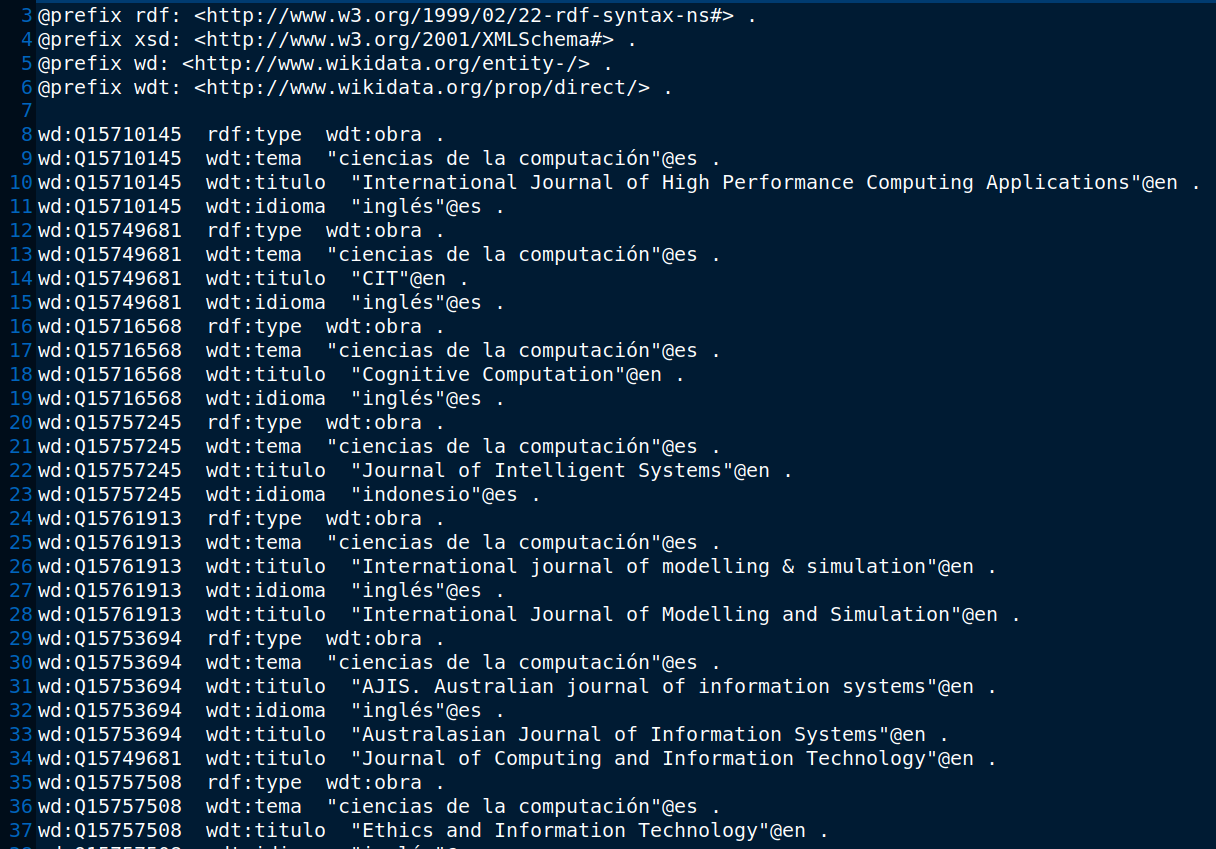
\includegraphics[scale=0.2]{imagenes/estruc_rdf_30.png} 
\caption{30 tripletas de la estructura RDF utilizada (ver archivo RDF.ttl) }
\end{figure} 

\begin{figure}[H]
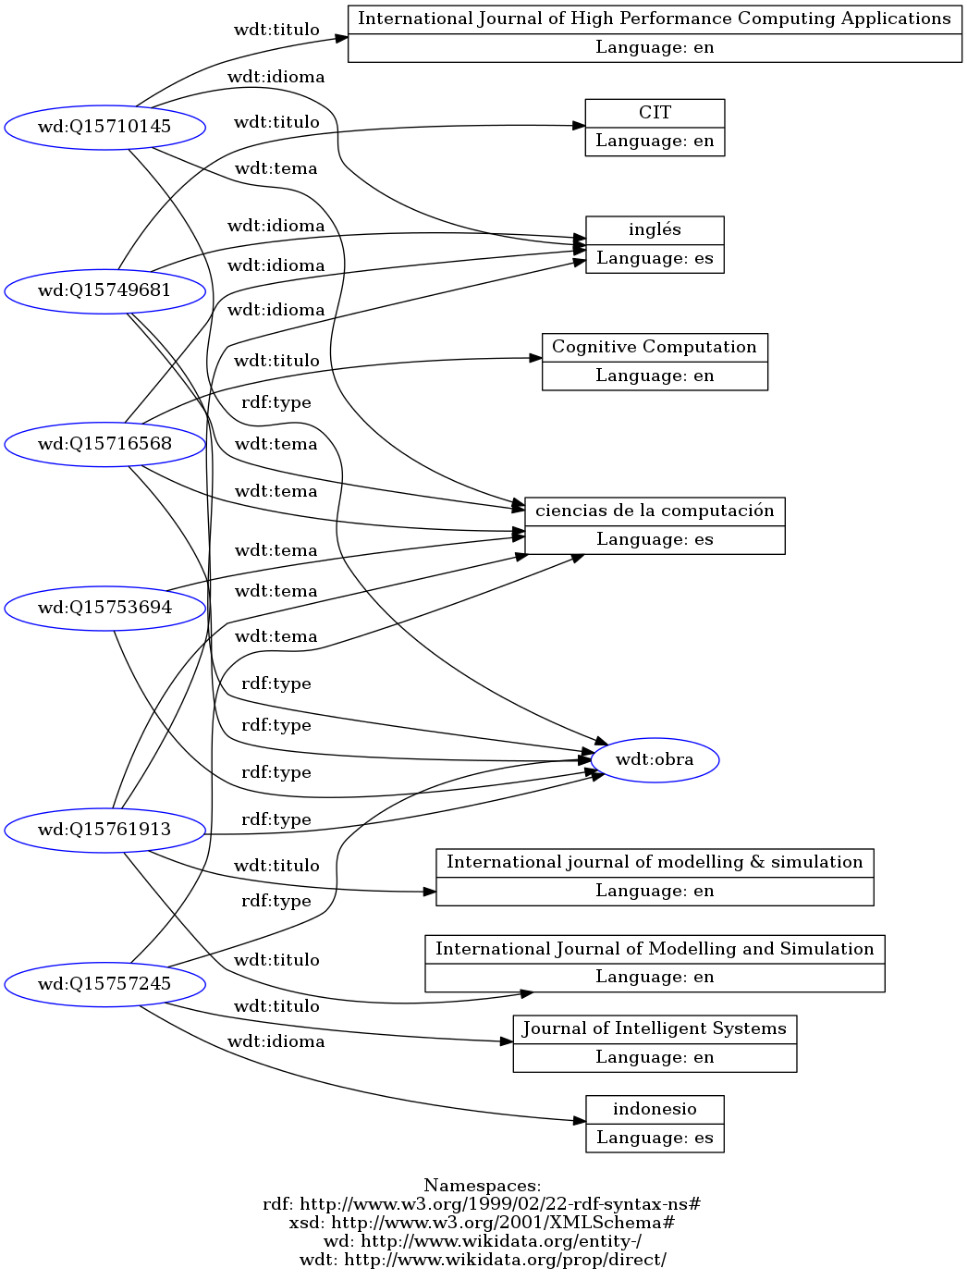
\includegraphics[scale=0.25]{imagenes/grafo_rdf_30.jpeg} 
\caption{Grafo generado con 30 tripletas de la estructura RDF utilizada \cite{b2}}
\end{figure} 

\vspace{0.2cm}

De acuerdo al art\'iculo, las principales diferencias entre el Transformer y el Transformer Universal consistn en que el Transformer Universal aplica el encoder para un n\'umero variable de pasos para cada token de entrada/salida (T pasos), mientras que el Transformador aplica exactamente $6$ capas de encoder/decoder, respectivamente. As\'i mismo, el Transformer Universal utiliza una representaci\'on de entrada ligeramente diferente: incluye un embedding de paso de tiempo adem\'as de la codificaci\'on posicional.

\vspace{0.2cm}

Los n\'umeros variables de pasos presentes en el Transformer Universal se logran mediante el uso de \textcolor{green}{Adaptive Computation Time}, un mecanismo propuesto por Alex Graves \cite{b6} que permite la aplicaci\'on del encoder y decoder un n\'umero variable de veces.
	
\vspace{0.2cm}

\subsection{Transformer-XL}

El transformer-XL es uno de los primeros modelos exitosos en abordar el problema de poseer una longitud fija en la secuencia de entrada. En el art\'iculo \textcolor{orange}{Transformer-XL: Attentive Language Models Beyond a Fixed-Length Context} \cite{b7} se propone este m\'etodo novedoso para el modelado de lenguaje, que permite que una arquitectura transformer aprenda dependencia a largo plazo, a trav\'es de un mecanismo de recurrencia, m\'as all\'a de una longitud fija sin alterar la coherencia temporal.

\vspace{0.2cm}

Se introduce un mecanismo recurrente a nivel de segmento que permite que el modelo reutilice estados ocultos anteriores en el momento del entrenamiento, abordando tanto los problemas del contexto de longitud fija como la fragmentaci\'on del contexto. En otras palabras, la informaci\'on hist\'orica se puede reutilizar y se puede extender tanto como lo permita la memoria de la GPU.
	
\vspace{0.2cm}

Para reutilizar adecuadamente los estados ocultos, los autores proponen un mecanismo llamado codificaciones posicionales relativas  que ayuda a evitar la confusi\'on temporal. Los modelos actuales no pueden distinguir la diferencia posicional entre entradas en diferentes segmentos en diferentes capas. La codificaci\'on de posici\'on relativa soluciona este problema al codificar el sesgo de informaci\'on posicional en los estados ocultos, que difiere de otros enfoques que realizan esto como el nivel de entrada.

\begin{figure}[h]
%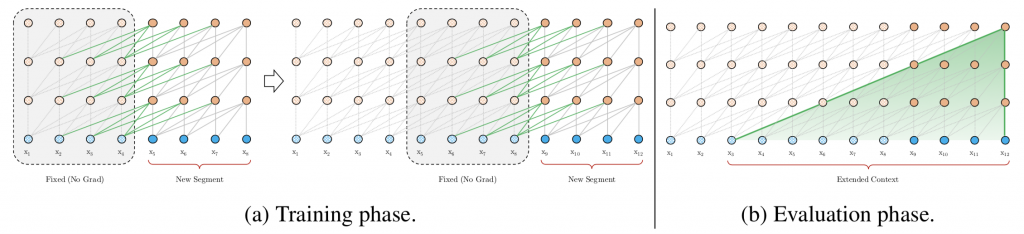
\includegraphics[scale=0.25]{imagenes/TransformerXL1.png} 
\caption{Transformer XL: Entrenamiento y Evaluación. Fuente: Transformer XL \cite{b7}}
\end{figure}


\vspace{0.2cm}


El transformer-XL reduce el puntaje de perplejidad SoTA anterior en varios conjuntos de datos como text8, enwiki8, One Billion Word y WikiText-103. Los autores afirman que el m\'etodo es m\'as flexible, m\'as r\'apido durante la evaluaci\'on (aceleraci\'on de $1874$ veces), se generaliza bien en conjuntos de datos peque\~nos y es eficaz para modelar secuencias cortas y largas.

\vspace{0.2cm}

As\'i mismo, los autores proponen una nueva m\'etrica llamada Relative Effective Context Length que proporciona una manera justa de comparar modelos que se prueban con mayores longitudes de contexto.

\subsection{XLNet}

XLNet es un modelo presentado en el art\'iculo \textcolor{green}{XLNet: Generalized Autoregressive Pretraining for Language Understanding} \cite{b8} que es un lenguaje autoregresivo que genera la probabilidad conjunta de una secuencia de tokens basada en la arquitectura del Transformer con recurrencia. Este modelo introduce una variante de modelado de lenguaje llamada modelado de lenguaje de permutaci\'on. Los modelos de lenguaje de permutaci\'on est\'an entrenados para predecir un token dado el contexto anterior como el modelo de lenguaje tradicional, pero en lugar de predecir los tokens en orden secuencial, predice los tokens en un orden aleatorio.

\vspace{0.2cm}

Adem\'as de usar el modelado de lenguaje de permutaci\'on, XLNet mejora BERT  al usar el Transformer XL como su arquitectura base. XLNet utiliza las dos ideas clave de Transformer XL: embeddings posicionales relativas y el mecanismo de recurrencia. Los estados ocultos del segmento anterior se almacenan en cach\'e y se congelan mientras se realiza el modelado del lenguaje de permutaci\'on para el segmento actual. Como todas las palabras del segmento anterior se usan como entrada, no es necesario conocer el orden de permutaci\'on del segmento anterior.
	
\subsection{BERT}

Este modelo \cite{b9},publicado el 2018, esta conformado por una pila de bloques Transformers, la cual esta pre-entrenada en un corpus de dominio general con 800 millones de palabras. 
Este modelo obtiene un mejor rendimiento que modelos anteriores a su publicación debido a su naturaleza bidireccional donde la atención se centra en toda la secuencia. 

\subsection{RoBERTa}

Es un modelo introducido en Facebook. El enfoque BERT robustamente optimizado RoBERTa \cite{b10}, es un reentrenamiento de BERT con una metodolog\'ia de entrenamiento mejorada, un $1000\%$ más de datos y potencia de cálculo. Para mejorar el procedimiento de entrenamiento, RoBERTa elimina tareas como Next Sentence Prediction (NSP) del entrenamiento previo de BERT e introduce el enmascaramiento dinámico para que el token enmascarado cambie durante las \'epocas de entrenamiento. 

\vspace{0.2cm}

RoBERTa supera a BERT y XLNet en los resultados de referencia de \href{https://gluebenchmark.com/}{GLUE}.

\subsection{DistilBERT}

Este modelo aprende una versión destilada (aproximada) de BERT, que retiene el $95\%$ de rendimiento pero utiliza solo la mitad del n\'umero de par\'ametros. Espec'ificamente, no tiene embeddings de tipo token, pooler y retiene solo la mitad de las capas del BERT de Google.

DistilBERT \cite{b11}, utiliza una técnica llamada destilation, que se aproxima a BERT de Google. La idea es que una vez que se ha entrenado una gran red neuronal, sus distribuciones de salidas completas se pueden aproximar usando una red más pequeña. Una de las funciones clave de optimización utilizadas para la aproximación posterior en las estadísticas bayesianas es la divergencia de Kulback-Leiber.

\section{Conclusiones}

\begin{itemize}
\item Se ha realizado clasificaci\'on multiclase utilizando la librer\'ia simpletransformers y modelos pre-entrenados, basados en BERT, obteniendo buenos resultados en m\'etricas de clasificaci\'on, especialmente del modelo distilBERT, que tiene un menor n\'umero de param\'etros que BERT y que utiliza el aprendizaje \texttt{teacher-students}, donde se entrena a una red de \texttt{students} para imitar la distribuci\'on de salida completa de la red del \texttt{teacher} (su conocimiento) y retiene el rendimiento de BERT.
\item En la tarea de traducci\'on, se realizaron comparaciones entre distintos modelos seq2seq y los modelos transformers, donde estos \'ultimos obtuvieron mejores resultados. Sin embargo el modelo Transformer XL modificado no logr\'o superar al Transformer original.
\end{itemize}

%\section{Referencias}
\begin{thebibliography}{00}
\bibitem{b1}\href{https://arxiv.org/abs/1502.03167}{https://www.w3.org/TR/rdf-sparql-query/}. 
\bibitem{b2}Página web para generar grafos a partir de una estructura RDF: \href{https://www.ldf.fi/service/rdf-grapher}.
\bibitem{b3} Jimmy Lei Ba, Jamie Ryan Kiros, Geoffrey E.Hinton. Layer Normalization (2016). Disponible en \href{https://arxiv.org/abs/1607.06450}{https://arxiv.org/abs/1607.06450}.
\bibitem{b4}Kishore Papineni , Salim Roukos , Todd Ward , Wei-jing Zhu (2002). BLEU: a Method for Automatic Evaluation of Machine Translation,  pp. 311-318. Proceedings of the 40th Annual Meeting of the Association for Computational Linguistics (ACL). 
\bibitem{b5}Mostafa Dehghani, Stephan Gouws, Oriol Vinyals, Jakob Uszkoreit, Łukasz Kaiser. Universal Transformers (2018). ICLR 2019. Disponible en \href{https://arxiv.org/abs/1807.03819}{https://arxiv.org/abs/1807.03819}
\bibitem{b6}Alex Graves. Adaptive Computation Time for Recurrent Neural Networks (2017). Disponible en \href{https://arxiv.org/abs/1603.08983}{https://arxiv.org/abs/1603.08983}.
\bibitem{b7}Zihang Dai, Zhilin Yang, Yiming Yang, Jaime Carbonell, Quoc V. Le, Ruslan Salakhutdinov. Transformer-XL: Attentive Language Models Beyond a Fixed-Length Context (2019). Disponible en \href{https://arxiv.org/abs/1901.02860}{https://arxiv.org/abs/1901.02860}. 
\bibitem{b8}Zhilin Yang, Zihang Dai, Yiming Yang, Jaime Carbonell, Ruslan Salakhutdinov, Quoc V. Le. XLNet: Generalized Autoregressive Pretraining for Language Understanding (2019). Disponible en \href{https://arxiv.org/abs/1906.08237}{https://arxiv.org/abs/1906.08237}.
\bibitem{b9}Jacob Devlin, Ming-Wei Chang, Kenton Lee, Kristina Toutanova. BERT: Pre-training of Deep Bidirectional Transformers for Language Understanding (2018). Disponible en \href{https://arxiv.org/abs/1810.04805}{https://arxiv.org/abs/1810.04805}.
\bibitem{b10}Yinhan Liu, Myle Ott, Naman Goyal, Jingfei Du, Mandar Joshi, Danqi Chen, Omer Levy, Mike Lewis, Luke Zettlemoyer, Veselin Stoyanov- RoBERTa: A Robustly Optimized BERT Pretraining Approach (2019). Disponible en \href{https://arxiv.org/abs/1907.11692}{https://arxiv.org/abs/1907.11692}.
\bibitem{b11}Victor Sanh, Lysandre Debut, Julien Chaumond, Thomas Wolf. DistilBERT, a distilled version of BERT: smaller, faster, cheaper and lighter (2019). Disponible en \href{https://arxiv.org/abs/1910.01108}{https://arxiv.org/abs/1910.01108}.
\bibitem{b12}Pytorch-Transform:Implementaci\'on de transformer para NLP. \href{https://pytorch.org/hub/huggingface\_pytorch-transformers/}{https://pytorch.org/hub/huggingface\_pytorch-transformers/}.
\bibitem{b13}Thomas Wolf, Lysandre Debut, Victor Sanh, Julien Chaumond,
Clement Delangue, Anthony Moi, Pierric Cistac, Tim Rault,
R\'emi Louf, Morgan Funtowicz, Jamie Brew. Transformers: State-of-the-art Natural
Language Processing (2019), HuggingFace Inc. Disponible en \href{https://arxiv.org/abs/1910.03771}{https://arxiv.org/abs/1910.03771}.
\bibitem{b14}SimpleTransformers \href{https://pypi.org/project/simpletransformers/}{https://pypi.org/project/simpletransformers/}.
\bibitem{b15} Xiang Zhang, Junbo Zhao, Yann LeCun. 
Character-level Convolutional Networks for Text Classification(2015). Disponible en \href{https://arxiv.org/abs/1509.01626}{https://arxiv.org/abs/1509.01626}. 
\bibitem{b16} Desmond Elliott, Stella Frank, Khalil Sima'an, Lucia Specia. 
Multi30K: Multilingual English-German Image Descriptions(2016). Disponible en \href{https://arxiv.org/abs/1605.00459}{https://arxiv.org/abs/1605.00459}. 
\bibitem{b17}TransformerXL from Scratch \href{https://github.com/keitakurita/Practical_NLP_in_PyTorch/blob/master/deep_dives/transformer_xl_from_scratch.ipynb}{notebook}.
\end{thebibliography}

\end{document}
